\documentclass[12pt,letterpaper]{article}

%%%%%%%%%%%%
% Includes %
%%%%%%%%%%%%
\usepackage[utf8]{inputenc}
\usepackage[margin=1 in]{geometry}
\usepackage{graphicx}
\usepackage{amsmath}
\usepackage{amsthm}
\usepackage{amsfonts}
\usepackage[justification=centering]{caption}

% Formatting
\renewcommand{\baselinestretch}{1.25}

% Theorems and other necessary structures
%\theoremstyle{definition}
\newtheorem{definition}{Definition}[section] % Definition
\newtheorem{theorem}{Theorem}[section] % Big result
\newtheorem{corollary}{Corollary}[theorem] % Follows from a theorem
\newtheorem{lemma}[theorem]{Lemma} % Minor result

% New commands
\newcommand{\R}{\mathbb{R}} % Real numbers
\newcommand{\N}{\mathbb{N}} % Natural numbers
\newcommand{\Z}{\mathbb{Z}} % Integral numbers

% Title information
\title{Compilers}
\author{2018A7PS0193P}

\begin{document}

\maketitle

\section{Process of Translation}

The process of compilers converting from source code (the high level language) to target code (the machine language) is known as translation.  It consists of many steps, which are described below.

\subsection{Lexical Analysis}

Lexical analysis follows the following steps:

\begin{enumerate}
\item Identify the valid set of characters in the language
\item Break the sequence of characters into appropriate words or tokens (keywords, numbers, operators, etc.)
\item Find out whether these tokens are valid or not.
\end{enumerate}

The key goal of the lexical analyzer is to break a sentence into a series of words/tokens. These breaks are generally done via certain separators. The tokens are recognized via some rules encoded into a Finite State Machine.

During the lexical phase, we may experience the following lexical errors:

\begin{itemize}
  \item Occurrence of illegal characters
  \item Exceeding the length of identifier
\end{itemize}

The output of the lexical analyzer will be a sequence of tokens and their ``type'', which signifies whether it is a identifier, operator, etc.

\subsection{Syntax Analysis}

The syntax analysis takes the sequence of tokens as an input, and generates a parse tree. In case the syntax is not correct according to the grammar rules, it flags a syntactical error. This is modelled using Context Free Grammars that will be recognized using PDAs or Table Driven processes.

\subsection{Semantic Analysis}

Semantic analysis takes the parse tree as an input, and outputs a disambiguated parse tree. It performs the following:

\begin{itemize}
  \item Check Semantics
  \item Error reporting (types, etc.)
  \item Disambiguate overloaded operators (meaning of operators depends on operands)
  \item Type coercion (type casting)
  \item Uniqueness checking (redeclaration of variables)
\end{itemize}

As such, the disambiguated parse tree gives us an unambiguous representation of the parse tree.

The phases mentioned till now comprise the \textbf{front end} of the compiler, where the source code is handled. After this, the compiler works on generating the target code.

\subsection{Code optimization}

This is an optional phase that modifies the programs to run faster and consume less resources like memory, registers, etc. However, it will not change the representation of the program.

Some examples of machine independent code optimization done is:

\begin{itemize}
  \item Common sub-expression elimination
  \item Copy Propagation
  \item Dead code elimination
  \item Code Motion
  \item Strength Reduction
  \item Constant Folding
\end{itemize}

\textit{TODO: See what these do and examples of each.}

\subsection{Code Generation}

This is the process of mapping from source level abstractions (identifiers, values, etc) to target machine abstractions (registors, memory, etc.). This is a two step process - initially, intermediate code gets generated from the disambiguated parse tree, which is used to generate the final machine code.

During code generation, we have to do the following:

\begin{itemize}
  \item Map identifiers to locations (memory or registers)
  \item Map source code operators to opcodes or sequences of opcodes.
  \item Transform conditionals and iterations to a test/jump or compare instructions
  \item We use layout parameter passing protocols - the locations for parameters, return values, etc.
\end{itemize}

\subsection{Post Translation Optimizations}

Unlike in the code optimization phase where we perform machine independent code optimizations, this does machine-dependent code optimizations. This is an optional phase as well, where we may remove unneeded operations or rearrange to prevent hazards. It is a flexible phase, and may occur at any time in the back-end of the compiler.

\subsection{Symbol Table}

The symbol table contains information required about the source program identifiers during compilation, including:

\begin{itemize}
  \item Category of variable
  \item Data type
  \item Quantity stored in structure
  \item Scope information
  \item Address in Memory
\end{itemize}

The symbol table must be present in every phase of the compiler, and is used in all the phases to get information about the identifiers.

\section{Advantages and Disadvantages of Compilers}

The advantages of compilers are:

\begin{itemize}
  \item Highly modular in nature
  \item It is retargetable. This means that if there is a single language and multiple machines, then we can use the same front end. If there are many languages
  \item Source code and machine independent optimizations are possible.
\end{itemize}

The limitations of the compiler are:

\begin{itemize}
  \item Design of programming languages has a huge effect on the performance of compilers.
  \item Lots of work is repeatable. For $S$ languages and $M$ machines, $S\cdot M$ compilers are needed. This is known as the $S*M$ problem of compilers.
\end{itemize}

The $S*M$ problem is generally solved by introducing some common intermediate language, called the \textbf{Universal Intermediate Language Generator}. Some common machine independent intermediate code generation techniques are:

\begin{itemize}
  \item Postfix Notation
  \item Three Address code
  \item Syntax tree
  \item Directed Acyclic Graph
\end{itemize}


\section{Lexical Analysis}

\subsection{Functions of the Lexical Analyzer}

The lexical analyzer performs the following functions:

\begin{itemize}
  \item Take high level language as input and output a sequence of tokens
  \item It generally cleans the code, by stripping off blanks, tabs newlines and comments.
  \item Keeps track of the line numbers for associated error messages
\end{itemize}

The lexical analyzer is modelled using regular expressions. As such, it's implementation is done with a DFA. An example of one rule is $L \cdot (L+D)^*$, where $L$ refers to a letter and $D$ refers to a digit.

\begin{definition}
  A token is a string of characters which logically belong together, e.g. keywords, number, identifiers, etc.
\end{definition}

\begin{definition}
  A pattern is the set of strings for which the same token is produced.
\end{definition}

\begin{definition}
  A lexeme is a sequence of characters matched by a pattern to form the corresponding token.
\end{definition}

Now that we understand the definitions, we can see what the lexical analyzer actually does - it transforms strings to the token and passes the lexeme as it's corresponding attribute. For instance, the integer 43 would become \texttt{<num,43>}.

\subsection{Working of the Lexical Analyzer}

The lexical analyzer reads the character one by one from the source code into the lexeme. When it reaches a separator, it assigns a token to the lexeme based on certain rules, and continues to read the characters once more.

However, reading the lexemes character by character is slow, and involves many IO operations. This is done from a buffer instead of directly from the file. Moreover, the prefix of a lexeme is often not enough to determine the token - think of the lexemes \texttt{=} and \texttt{==}. We instead use a lookahead pointer to determine the appropriate token for a lexeme, and then push back the characters that we do not need in the current lexeme.

\subsection{Symbol Table and the Lexical Analyzer}

The lexical analyzer also interfaces with the symbol table. When the lexical analyzer discovers a lexeme constituting an identifier, it enters that lexeme to the symbol table. Sometimes, information regarding the token of a particular lexeme may also be store in the symbol table. As such, the symbol table must implement the following operations:

\begin{enumerate}
  \item \texttt{insert(s,t)} : Save lexeme \texttt{s} and token \texttt{t} and return pointer.
  \item \texttt{lookup(s)} : return the index of entry for lexeme \texttt{s} or \texttt{`0'} if \texttt{s} is not found.
\end{enumerate}

To make the symbol table space efficient, we save lexemes in some separate memory, and instead store pointers to the lexemes in the symbol table.

The rule for identifying an identifier and a keyword is generally the same. To be able to tokenize the identifiers and keywords separately, we initialize the symbol table with the list of keywords, say, by calling \texttt{insert("if",keyword)}.

\subsection{Challenges in Development of Lexical Analyzer}

\begin{itemize}
  \item \textbf{Free vs Fixed Lexemes} : A language could specify that lexemes must be in a free or a fixed format. For instance, in a free format, code could look like this.
    \begin{verbatim}
    flag = flag
    * 6;
    \end{verbatim}
    But in the case of fixed format, this must be entirely in one line. An example of a fixed format language is Python, while a free format language is C.
  \item \textbf{Whitespaces} : How do we deal with whitespaces? Some languages ignore whitespaces until a separator is reached (or interpret contextually), while some languages consider the whitespaces as separators themselves. The former is much more complicated to implement than the latter.
  \item \textbf{Maximal Munch} : The principle of maximal munch directs the lexical analyzer to consume as much available input as possible while creating a construct. This allows us to deal with lexemes like \texttt{iff}, and correctly assign it as a identifier rather than the keyword \texttt{if}.
\end{itemize}

\subsection{Techniques for specifying tokens} 

\begin{definition}
  Consider $R_i$ is a regular expression and $N_i$ is a unique name, then a regular definition is a series of definitions of the following form 
  \[N_1 \rightarrow R_1 \]
  \[N_2 \rightarrow R_2 \]
  \[...\]
  \[N_n \rightarrow R_n \]
  where each $R_i$ is a regular expression over $\sum \bigcup \{N_1,N_2,...N_n\}$.
\end{definition}

Hence, by assigning a special name $N_i$ to the regular expression $R_i$, we are in effect defining macros, that remove redundancy in later parts.

The following is an example regular definition for identifiers:

\[\text{Alphabet} \rightarrow A|B|C|...Z|a|b|c|...|z\]
\[\text{Digit} \rightarrow 0|1|2|...|9\]
\[\text{Identifier} \rightarrow \text{Alphabet}(\text{Alphabet} | \text{Digit})^*\]

This too comes with its own challenges. Regular expressions often fail when identifying the appropriate token, and may pass the invalid tokens to the subsequent translation phases of the compiler (how?). They are only language specifications. Tokenization is a implementation problem.

Tokenization can be done via the following steps:

\begin{enumerate}
  \item Construct regular expressions for lexemes of each token
  \item Construct $R$ matching all lexemes of tokens, so $R = R_1+R_2+...$, in some well defined precedence order.
  \item Consider the input stream to be $S=s_1s_2...s_n$. For $i \in [1,n]$, verify whether $s_1...s_i \in L(R)$.
  \item If $s_1...s_i \in L(R) \implies s_1..s_i \in L(R_x)$ for some $x$. We choose the smallest $x$ to be the class of $s_1..s_i$. 
  \item Discard the tokenized input and go back to step 3.
\end{enumerate}

The procedure gives preference to tokens specified earlier using regular expressions. If $s_1..s_i \in L(R)$ and $s_1...s_j \in L(R)$, we choose the longest prefix, in accordance with the principle of maximal munch.

To implement our regular definitions and recognize tokens, we use \textbf{transition diagrams}. They are shown diagrammatically in the same way as Finite Automata. Transitions can be labelled with a symbol, a group of symbols, or regular definitions. A few states may be \textbf{retracting states} that indicates that the lexeme does not include the symbol that can bring us to the accepting state.

Sometimes, we may want to push back extra characters into the token stream (think of \texttt{>} and \texttt{>=}, we may want to push back the extra character read if the token is \texttt{>}). We mark those states with a \texttt{*}, to show that we must push back extra characters.

\subsubsection{Example for Hexadecimal and Octal constants}

The regular definition would be:

\[hex \rightarrow 0|1|2|...|9|A|B|C|...F\]
\[oct \rightarrow 0|1|2|...|7\]
\[Qualifier \rightarrow u|U|l|L\]
\[OctalConstant\rightarrow 0 oct^+(Qualifier|\epsilon)\]
\[HexadecimalConstant\rightarrow 0(x|X)hex^+(Qualifier|\epsilon)\]

The transition diagram for the given regular definition is given in Fig 1.

\begin{figure}[htpb]
  \centering
  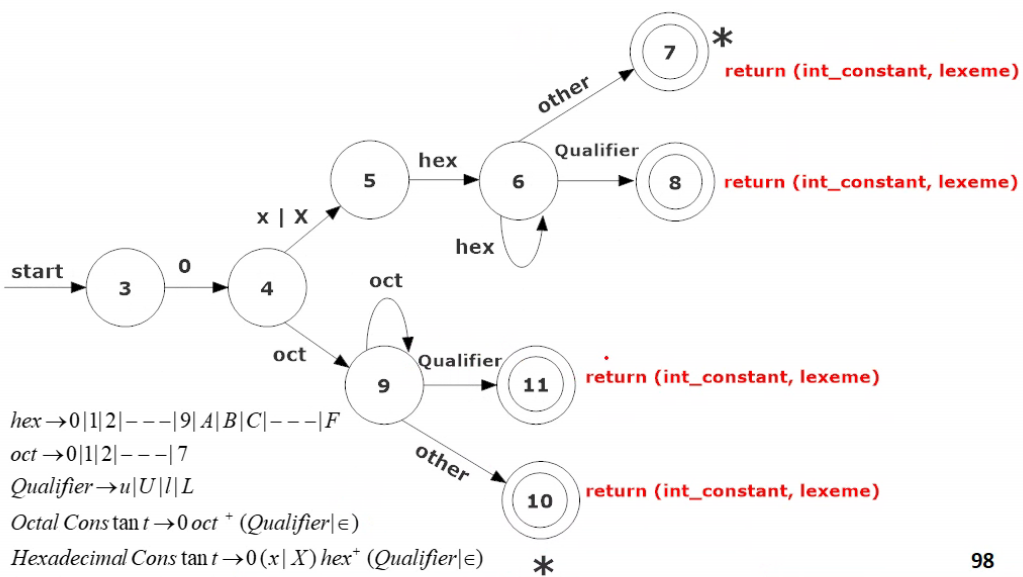
\includegraphics[width=0.8\linewidth]{./assets/hex_oct_trans_diag.png}
  \caption{Transition diagram for the Hex and Octal constants}%
  \label{fig:}
\end{figure}

The retracting states are not given. If we get a ``bad character'', we should report it as a lexical error.

\subsubsection{Example for Unsigned numbers}

The regular definition is:

\[Digit \rightarrow 0|1|2|...|9\]
\[Digits \rightarrow Digit^+\]
\[Fraction \rightarrow '.'Digits|\epsilon\]
\[Exponent \rightarrow (E(+|-|\epsilon)Digits)|\epsilon\]
\[Number \rightarrow Digits \cdot Fraction \cdot Exponent\]

The resulting transition diagram from this is in Fig 2.

\begin{figure}[htpb]
  \centering
  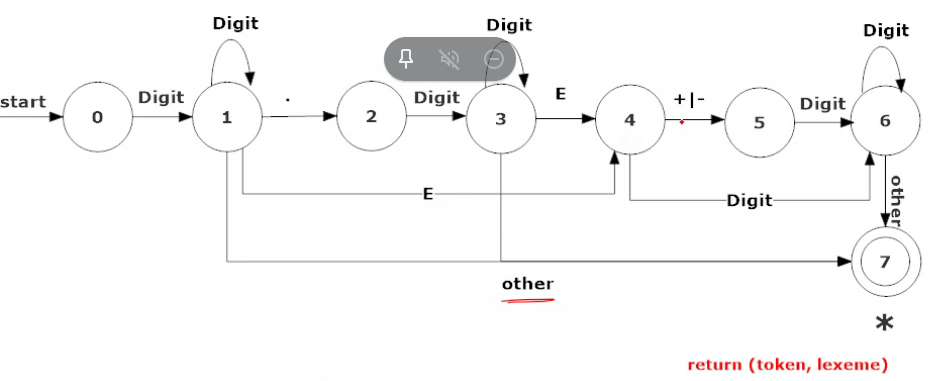
\includegraphics[width=0.8\linewidth]{./assets/unsigned_num_trans_diag.png}
  \caption{Transition Diagram for Unsigned Numbers}%
  \label{fig:}
\end{figure}

The issue here is this often introduces a lot of complexity. Instead, we may add split this into multiple transition diagrams, to improve implementation complexity. This also empirically better speeds. These multiple transition diagrams can be appropriately combined to generate a lexical analyzer.

\end{document}
